\section{Theoretical Foundations}
\subsection{The hard problem of consciousness}
Chalmers (1995) formulated the hard problem as follows: no combination of physical quantities, however complex, logically entails the existence of subjective experience. Every physical description --- neuronal, computational, functional --- describes what the brain does. It does not describe what it is like to be a brain. It does not describe why experience exists. What I propose: consciousness is not generated by the brain. The brain is a receiver. Experience is the transduction of the akashic field.

\subsection{Russellian Monism}
Russell (1927) observed something profound: physics describes the structural properties of matter --- mass, charge, spin, location --- but is entirely silent about the intrinsic nature of that which carries these properties. Let S be any physical system: R(S) denotes its relational/structural properties and I(S) its intrinsic properties. The Russellian thesis says that I(S) is proto-experiential for any S.

\subsection{Integrated Information Theory}
Tononi (2004, 2008) offers a mathematical framework for quantifying consciousness:
\begin{equation}
\Phi = \min_{\{P \in P\}} D_{KL}(p(X_{t+1})|X_{t}) \parallel \prod_{i} p(x_{i} \land (t+1)|x_{i} \land t))
\end{equation}
A simple explanation: $\Phi$ measures how integrated the information in a system is. The larger $\Phi$ is, the richer the system's experience.

\subsection{Orchestrated Objective Reduction}
Penrose (1996) proposes that quantum superpositions undergo spontaneous gravitational collapse when the superposition energy $E_G$ reaches a threshold:
\begin{equation}
\tau \approx \frac{\hbar}{E_G}
\end{equation}
What interested me: the collapse frequency for cortical microtubules is $\tau \approx 25$ ms, corresponding to $\sim 40$ Hz --- exactly the frequency of gamma oscillations, the most robust empirical marker of conscious states. Experimental support: Babcock et al. (2024) showed ultraviolet superradiance in microtubules at room temperature; Kalra et al. (2023) showed that anaesthetic gases specifically attenuate quantum optical effects in microtubules.

\subsection{Kaluza--Klein and F-theory}
Theodor Kaluza proposed in 1919 the unification of gravity with electromagnetism by means of a fifth dimension. Einstein was enthusiastic and worked on this theory between 1938 and 1943. The original formulation:
\begin{equation}
dS^2 = g_{\mu\nu} dx^\mu dx^\nu + \varphi^2(dx^5 + A_{\mu} dx^\mu)^2
\end{equation}

\subsection{The Akasha field}
The concept of Akasha (Sanskrit: \emph{ākāśa}) is a fundamental element in Indian philosophy. Akasha is the subtlest element, immaterial. It was the first to manifest in the universe. All the other elements are said to have developed from it. In theosophy, Akasha is reinterpreted as a universal information field (Laszlo, 2014). The ``Akashic Record'' records every event in the universe. The ART-12D hypothesis: Akasha is the quantum field of dark matter. \textit{Note: Akasha is used here only as a metaphor for a physical field, not as a religious entity.}

\subsection{Grey matter vs. dark matter}
Grey matter is the tissue of the central nervous system made up mainly of neuronal cell bodies, dendrites, unmyelinated axon terminals and glial cells. It is the seat of information processing. White matter is made up of myelinated axons and is responsible for transmission.

\subsection{An operational definition of consciousness}
I propose an operational definition that separates the content of consciousness from the capacity to integrate it:
\begin{equation}
C_{\text{total}} = I_{\text{content}} \times C_{\text{awareness}}
\end{equation}
where $I_{\text{content}}$ is structured information (the content of experience) and $C_{\text{awareness}}$ is awareness (the capacity to know that you know). Think of a camera. It captures images (information), but it does not know that it captures them. A person with a camera captures images AND knows that they are capturing them. In the same way, consciousness is information + awareness.

\subsection{Convergence with Dulcan}
Dumitru Constantin Dulcan (b. 1938), a neurologist and psychiatrist, published ``The Intelligence of Matter'' in 1981, which was awarded the ``Vasile Conta'' prize for philosophy of the Romanian Academy in 1992. The ideas that influenced me: consciousness is not generated by the brain but uses it as an instrument; the subconscious contains the infinite intelligence of the Universe; thought is the most powerful force in the universe, with a frequency and an energy field of its own; there is a field of energy and light that coordinates matter. The convergence with ART-12D: Dulcan provides the conceptual intuition, ART-12D provides the mathematical formalisation and the testable predictions.

\subsection{The tripartite structure of the human entity}
I propose a tripartite model of the human entity, analogous to the states of aggregation of water:
\begin{table}[H]
\centering
\begin{tabular}{@{}llll@{}}
\toprule
\textbf{State of aggregation} & \textbf{Human entity} & \textbf{Substrate} & \textbf{ART-12D counterpart} \\ \midrule
Solid & Physical body & Matter & M (ordinary matter) \\
Liquid & Soul & Energy & E (the field of consciousness) \\
Gas & Spirit & Information & Sp (the akashic field) \\ \bottomrule
\end{tabular}
\end{table}
Formalisation: $H = M + E + Sp$. Consequences: death does not destroy the entity, it only changes the dominant state of aggregation; consciousness can access any of the three states; illness appears when one of the states is unbalanced.

\subsection{The forms of thought as informational structures}
Thoughts are not merely neuronal activity but informational structures that can take multiple forms. Imagined (internal visualisation, the field of consciousness), spoken (the spoken word, the akashic field + a sound wave), written (written text, matter + information), drawn (visual representation, matter + form). General formalisation: $F_{\text{thought}} = \sum_{\text{forms}} \alpha_i F_i$.

\subsection{Empathy as frequency resonance}
Empathy can be formalised as a particular case of telepathy, in which the coupling is emotional rather than informational. Formalisation:
\begin{equation}
\text{Empathy}(A,B) = \frac{1}{1 + \frac{(\omega_A - \omega_B)^2}{\Gamma^2}}
\end{equation}
Interpretation: when the frequencies coincide ($\omega_A = \omega_B$) empathy is maximal; when the frequencies differ, empathy decreases; empathy does not depend on distance (the field is omnipresent). A testable prediction: couples with high empathy should show stronger EEG correlations than couples with low empathy.

\subsection{The word as an excitation of the akashic field}
I propose that dark matter has an acoustic manifestation --- a spectrum of oscillations that can be excited by sound waves. The cosmological motivation: the primordial acoustic oscillations (BAO) are fluctuations in matter density that propagated as sound waves in the early universe. In ART-12D these oscillations are oscillations of the akashic field. Formalisation:
\begin{equation}
A(x,t) = \sum_n A_n \cos(\omega_n t + \varphi_n)
\end{equation}
The acoustic spectrum:
\begin{equation}
\omega_n = \frac{1}{R} \sqrt{n^2 + \mu_A^2 R^2}
\end{equation}
The word--field coupling:
\begin{equation}
L_{\text{int}} = g_{\text{sound}} A \cdot \Phi_{\text{sound}}
\end{equation}
Differentiated effects: Love (200-400 Hz, activates the positive emotional areas), Fear (500-800 Hz, activates the amygdala), Healing (300-500 Hz, activates positive expectation), Death (150-300 Hz, activates the anxiety areas).

\textbf{The scale problem.} The acoustic spectrum $\omega_n$ is fixed by the same compactification radius that gives dark matter its mass. For $1/R = 10^{-5}$ eV the modes sit at GHz, not at hundreds of Hz. A resonance at 150--800 Hz would require $1/R \approx 1.24\times10^{-12}$ eV, roughly seven orders of magnitude below the mass scale. Until a second compactification scale is introduced, the prediction has no numerical content: the coupling $g_{\text{sound}}$ is not fixed independently.

\begin{figure}[H]
\centering
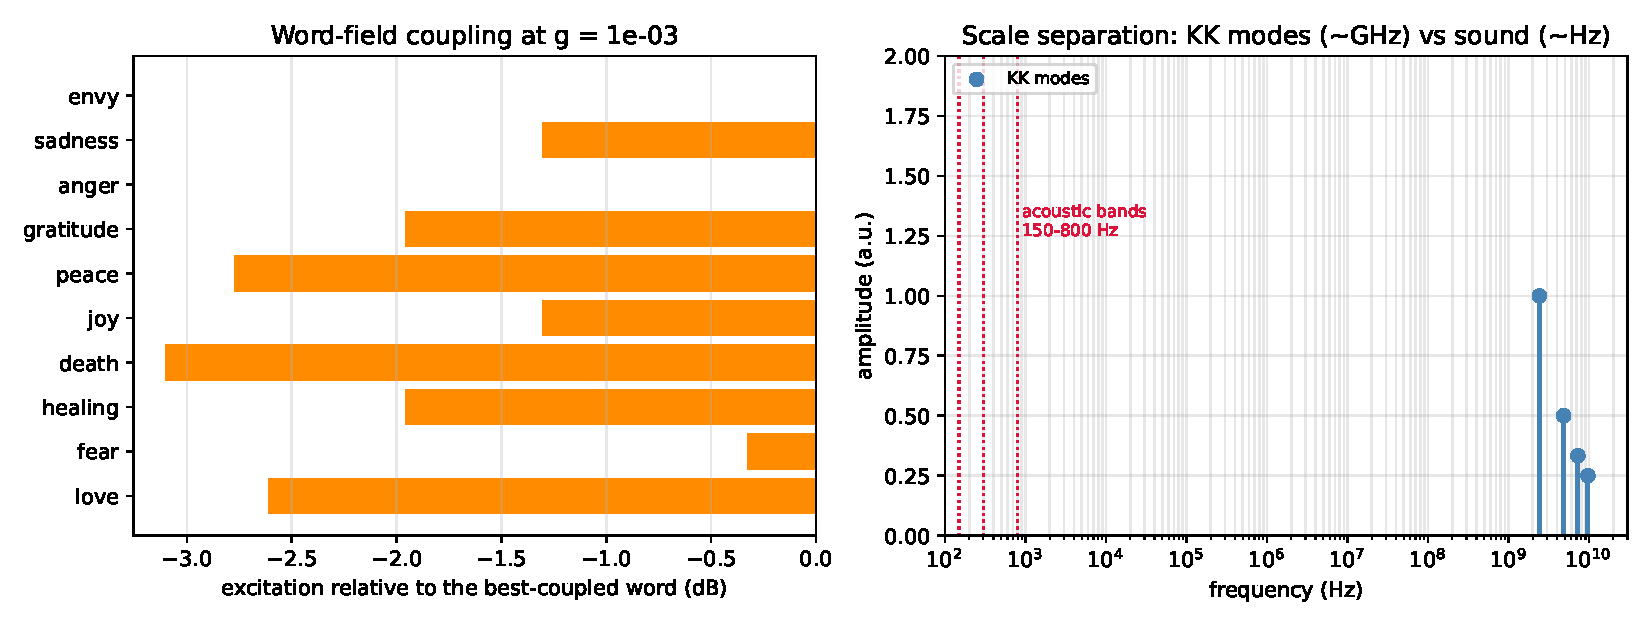
\includegraphics[width=0.9\textwidth]{figures/fig06_word_excitation.pdf}
\caption{Left: the relative word--field coupling for the ten bands used in the paper. Right: the scale separation between the KK modes (~GHz) and the acoustic bands (~Hz).}
\label{fig:cuvant}
\end{figure}

\subsection{Time as vibration}
The definition of the second: ``One second is the duration of 9,192,631,770 periods of the radiation of the caesium-133 atom.'' What happens if the frequency changes: if the frequency rises, time is compressed; if the frequency falls, time is dilated. The Schumann resonance: historically $\sim 7.83$ Hz, recently $\sim 12$ Hz. The heart as a biological clock: fear ($\sim 120$ bpm) --- time flies; meditation ($\sim 50$ bpm) --- time is dilated; deep sleep ($\sim 40$ bpm) --- time disappears. Relative, not absolute, references: caesium (9,192,631,770 Hz), Schumann (7.83-12 Hz), the heart (1.2 Hz). They are all relative. None of them is ``the true one''.
\begin{equation}
\text{Reality} = \frac{\text{Change}}{\text{Reference}}
\end{equation}

\subsection{Multiple realities and the multiverse}
The total akashic field: $A_{\text{total}} = \sum_{k=1}^{N_{\text{vacua}}} A_k$. The state of the multiverse: $|\Psi_{\text{multiverse}}\rangle = \otimes_{k=1}^{N_{\text{vacua}}} |A_k\rangle$. The intersection of realities: realities are not merely parallel --- they can intersect.

\subsection{The universal library (Akasha)}
The content of the field: the akashic field contains all information --- everything that was, everything that is, everything that will be.
\begin{equation}
A_{\text{total}} = \sum_{\text{(all events)}} A_i
\end{equation}
Access to information:
\begin{equation}
I_{\text{access}}(t) = \int_0^\infty S_A(\omega) S_G(\omega, t) d\omega
\end{equation}
Indexing: information is indexed by relevance, not by time.
\begin{equation}
\text{Information received} = \text{Akashic field} \times \text{Relevance}(t)
\end{equation}

\subsection{The hierarchy of reception}
\begin{table}[H]
\centering
\begin{tabular}{@{}clcc@{}}
\toprule
\textbf{Level} & \textbf{System} & \textbf{$\Phi$} & \textbf{Access} \\ \midrule
0 & Thermostat & 0 & None \\
1 & C. elegans & Minimal & Chemotaxis \\
2 & Insect & Low & Sensation \\
3 & Mouse & Moderate & Emotion \\
4 & Dog & High & Empathy \\
5 & Corvid & High & Planning \\
6 & Octopod & Distributed & Problem solving \\
7 & Human & Very high & Self-reference \\
8 & Trained human & Extended & Metacognition \\ \bottomrule
\end{tabular}
\end{table}
The limit of reception: $\lim_{\Phi \rightarrow \infty} E(\Phi) = I_{\text{total}}$.

\subsection{The Word as origin: the convergence of religions}
All the great religious traditions describe the Word as the origin of the universe. Christianity has the Logos --- the Word (the fundamental mode of the field). Hinduism has Om (the primordial vibration). Islam has Kun (``Be!'').

\subsection{The acoustic manifestation of the akashic field}
$A(x,t) = \sum_n A_n \cos(\omega_n t + \varphi_n)$. The acoustic spectrum: $\omega_n = \frac{1}{R} \sqrt{n^2 + \mu_A^2 R^2}$.

\subsection{God in ART-12D}
There are four hypotheses. God is the akashic field itself. God is the source of the field. God is universal consciousness. God is a human projection. I do not know which one is correct. But the question is legitimate.

\subsection{Dark matter and dark energy: two faces of the same field}
The ART-12D hypothesis: dark matter and dark energy are two aspects of the same akashic field. Formalisation:
\begin{equation}
L_A = \frac{1}{2} g^{MN} \partial_M A^* \partial_N A + \frac{1}{2} \mu_A^2 |A|^2 - \frac{\lambda_A}{4} |A|^4
\end{equation}
The equation of state: $w = p_A / \rho_A$. For an oscillating field the time average is computed exactly along the orbit and depends on the ratio $\delta = A_{\text{osc}}/A_{\min}$ between the oscillation amplitude and the value of the potential at its minimum. There are three distinct regimes:
\begin{center}
\begin{tabular}{@{}lll@{}}
\toprule
\textbf{Regime} & \textbf{Condition} & $w$ \\ \midrule
Small oscillation about the minimum & $\delta \ll 1$ & $0$ (matter) \\
Oscillation dominated by the quartic term & $\delta \gg 1$ & $1/3$ (radiation) \\
Field frozen at the minimum & $\delta = 0$ & $-1$ (cosmological constant) \\ \bottomrule
\end{tabular}
\end{center}
Version 30 claimed that the large-amplitude regime gives $w \simeq 1$. The correct value is $1/3$: the virial theorem gives $\langle K \rangle = 2\langle V \rangle$ for a quartic-dominated potential. The value $w = 1$ corresponds to kinetic dominance (kination), which the quartic oscillations do not reach, while $w = -1$ corresponds to the frozen field, not to small amplitude.
